\subsection{Режим счётчика}
\selectlanguage{russian}

\begin{figure}[bt]
	\centering
	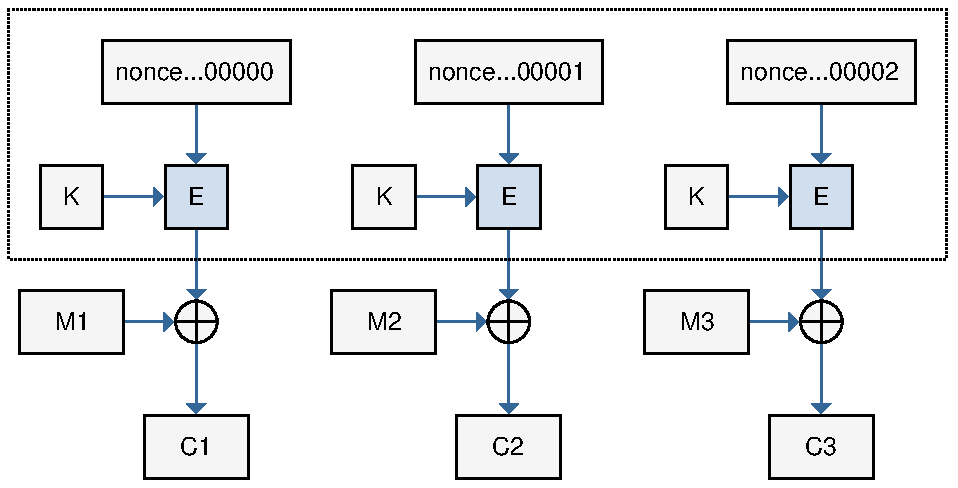
\includegraphics[width=1\textwidth]{pic/CTR}
	\caption{Режим счётчика. Пунктирной рамкой выделена область формирования \emph{гаммы}, независящей от открытого текста.}
	\label{fig:CTR}
\end{figure}

В режиме счётчика (\langen{Counter, CTR}, рис.~\ref{fig:CTR}) правило шифрования имеет вид, похожий на режим обратной связи по выходу (OFB), но позволяющий вести независимое (параллельное) шифрование и расшифрование блоков:
\[ \begin{array}{l}
    K_j = E_K(\textrm{Nonce} ~\|~ j - 1), ~ j = 1, 2, \dots, n, \\
    C_j = M_j \oplus K_j,
\end{array} \]
где $\textrm{Nonce} ~\|~ j - 1$ -- конкатенация битовой строки одноразовой метки $\textrm{Nonce}$ и номера блока, уменьшенного на единицу.
%Для стандарта AES значение $\textrm{Nonce}$ занимает 16 бит, номер блока -- 48 бит. С одним ключом выполняется шифрование $2^{48}$ блоков.

Правило расшифрования идентичное:
\[ \begin{array}{l}
    M_j = C_j \oplus K_j. \\
\end{array} \]
